\documentclass{beamer}

%packages:
% \usepackage{tfrupee}
% \usepackage{amsmath}
% \usepackage{amssymb}
% \usepackage{gensymb}
% \usepackage{txfonts}

% \def\inputGnumericTable{}

% \usepackage[latin1]{inputenc}                                 
% \usepackage{color}                                            
% \usepackage{array}                                            
% \usepackage{longtable}                                        
% \usepackage{calc}                                             
% \usepackage{multirow}                                         
% \usepackage{hhline}                                           
% \usepackage{ifthen}
% \usepackage{caption} 
% \captionsetup[table]{skip=3pt}  
% \providecommand{\pr}[1]{\ensuremath{\Pr\left(#1\right)}}
% \providecommand{\cbrak}[1]{\ensuremath{\left\{#1\right\}}}
% %\renewcommand{\thefigure}{\arabic{table}}
% \renewcommand{\thetable}{\arabic{table}}      

\setbeamertemplate{caption}[numbered]{}

\usepackage{enumitem}
\usepackage{tfrupee}
\usepackage{amsmath}
\usepackage{amssymb}
\usepackage{graphicx}
\usepackage{txfonts}

\def\inputGnumericTable{}

\usepackage[latin1]{inputenc}                                 
\usepackage{color}                                            
\usepackage{array}                                            
\usepackage{longtable}                                        
\usepackage{calc}                                             
\usepackage{multirow}                                         
\usepackage{hhline}                                           
\usepackage{ifthen}
\usepackage{caption} 
\captionsetup[table]{skip=3pt}  
\providecommand{\pr}[1]{\ensuremath{\Pr\left(#1\right)}}
\providecommand{\cbrak}[1]{\ensuremath{\left\{#1\right\}}}
\renewcommand{\thefigure}{\arabic{table}}
\renewcommand{\thetable}{\arabic{table}}   
\newcommand*{\Comb}[2]{{}^{#1}C_{#2}}
\providecommand{\brak}[1]{\ensuremath{\left(#1\right)}}
\newcommand{\mydet}[1]{\ensuremath{\begin{vmatrix}#1\end{vmatrix}}}
\providecommand{\cbrak}[1]{\ensuremath{\left\{#1\right\}}}
\providecommand{\sbrak}[1]{\ensuremath{{}\left[#1\right]}}
% Theme choice:
\usetheme{CambridgeUS}

% Title page details: 
\title{Assignment 8} 
\author{Pericherla Pranav Varma\\CS21BTECH11044}
\date{\today}
% \logo{\large \LaTeX{}}


\begin{document}

    % Title page
    \begin{frame}
        \titlepage 
    \end{frame}

    % Outline
    \begin{frame}{Outline}
        \tableofcontents
    \end{frame}

    \section{Question}
    	\begin{frame}{Question}
    	Papoulis Pillai Ch5 Ex 8-27:\\[9pt]
    The weights of cereal boxes are the values of a random variable x with mean $\eta$. We measure
64 boxes and find that x = 7.7 oz. and s = 1.5 oz. Test the hypothesis $H_o$: $\eta$ = 8 oz. against
$H_1$: $eta \neq 8$oz. with $\alpha$ = 0.1 and $\alpha$ = 0.01.
    	\end{frame}
%    
    \section{Solution}
        \begin{frame}{Solution}
        From Hypothesis testing,\\
        Critical region $\mydet{x - {\eta}_0} > {t}_{1 - \alpha /2 } (n-1) \dfrac{s}{\sqrt{n}}$ \\[9pt]
        $q_u = t_u(n-1)$\\[9pt]
        (i) \underline{$\alpha = 0.1$}
        \begin{align*}
        t_{1 - \alpha /2} (n-1) &= t_{1 - 0.05} (64 - 1) = t_{0.95} (63) = 1.67\\[9pt]
        \mydet{x-8} &> 1.67 \times 1.5/8 =0.313\\
        \end{align*}
        Thus interval of $x = 8 \pm 0.313$ \\
        \end{frame}
    %
    \begin{frame}{Solution}
    Since the $ x = 7.7 $ lies in interval of $8 \pm 0.313$ \\[7pt]
    \underline{we accept $H_0$}\\[9pt]
    (ii) \underline{$\alpha = 0.01$}
    \begin{align*}
     t_{1 - \alpha /2} (n-1) &= t_{1 - 0.005} (64 - 1) = t_{0.995} (63) = 2.62\\[9pt]
     \mydet{x-8} &> 2.62 \times 1.5/8 =0.49\\
    \end{align*}
    Thus interval of $x = 8 \pm 0.49$ \\
    \end{frame}
    %
    \begin{frame}{Solution}
    Since $x = 7.7$ is inside the interval of $8 \pm 0.49$\\[7pt]
    \underline{We accept $H_0$}
    \begin{figure}[H]
		\centering
			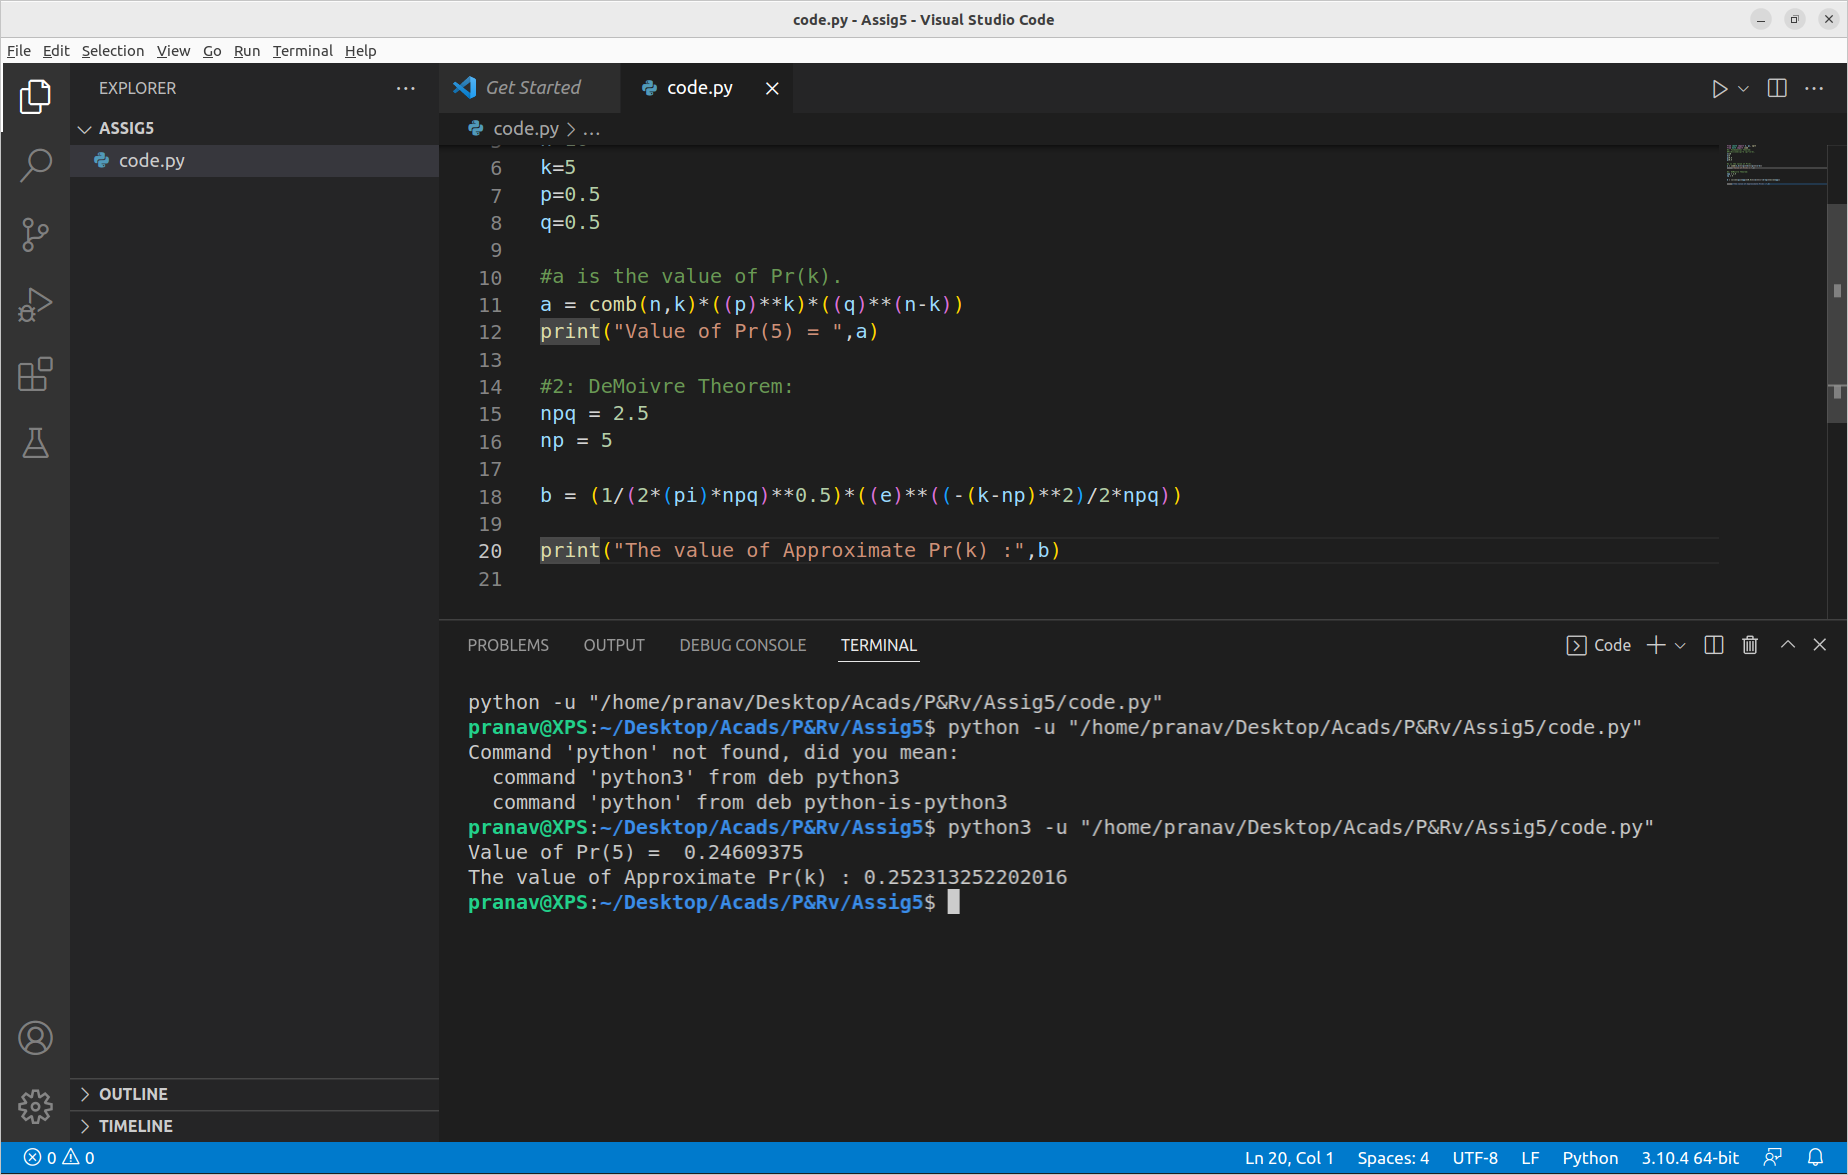
\includegraphics[width=\columnwidth]{figs/output.png}
			\caption{Verification Code}
			\label{Fig1}	
	\end{figure}
    \end{frame}
    
    
\end{document}